\documentclass[a4paper,12pt]{report}
\usepackage[slovak,english]{babel}
\usepackage[T1,IL2]{fontenc}             
\usepackage[utf8]{inputenc}    
\usepackage{amsmath}
\usepackage{amssymb,amsfonts,amscd}
\usepackage{array,hhline}
\usepackage{makeidx}
\usepackage{fancyhdr}
\usepackage{graphicx}
\usepackage{listings}
    %%\usepackage{titlepage}
    %%\usepackage{multicol}
\usepackage{eurosym}
\usepackage{url,mathptmx} 
\usepackage[pdftex,unicode,bookmarks=false]{hyperref}
\usepackage{comment}



\renewcommand{\baselinestretch}{1.5}  % pre zvascenie riadkovania

\addtolength{\oddsidemargin}{-.5cm}
\addtolength{\evensidemargin}{-2.9cm}   
\addtolength{\topmargin}{0cm}
\addtolength{\textheight}{0pt}
\addtolength{\textwidth}{2.cm}
\addtolength{\textheight}{2.cm}
\newlength{\verbcorr}
\setlength{\verbcorr}{0ex}



\begin{document}
\selectlanguage{slovak}


\pagestyle{empty}
\pagenumbering{arabic}

\hypersetup{pageanchor=false} 

\begin{titlepage}
\phantom.

\bigskip

\begin{center}
{\sc\LARGE Žilinská Univerzita v Žiline}
\medskip

{\sc\Large Fakulta riadenia a informatiky}

\vfill\vfill\vfill\vfill

{\sc\LARGE Bakalárska práca}

\medskip

{\large Študijný odbor: {\bf Informatika}}
\end{center}


\vfill\vfill\vfill\vfill


\phantom.\hfill

\begin{center}
{\large\bf Oľga Chovancová}

\medskip

{\large\bf Vizualizácia dát získaných pomocou SCADA systémov s využitím HTML 5 štandartov}

\medskip

Vedúci: {\bf Ing. Juraj Veverka}\\
Tútor	\textbf{Ing. Patrik Hrkút, PhD.}
\medskip
 
\hfill
Reg.č. 5/2014
\hfill
Máj 2015
\hfill\phantom.
\end{center}

\hspace{1.7cm}\phantom.

\vspace{2.9cm}

\phantom.
\end{titlepage}
%%%%%%%%%%%%%%%%%%%%%%%%%%%%%%%%%%%%%%%%%%%%%%%%%%%%%%%%%%%%%%%%%%%%%%%%%%%%%%%%%%%%%%%%%%%%%%%%%%%%%%%%%%%%%%%%%%%%%%%%%%%%%%%%%%%%%%%%%%%%%%%%%%%%%%%%%%%%%%%%%%%%%%%%%%%%%%%%%%%%%%%%%%%%%%%%%%%%%%%%%%%%%%%%%%%%%%%%%%%%%%%%%%%%%%%%%%%%%%%%%%%%%%%%%%%%%%%%%%

%%%%%%%%%%%%%%%%%%%%%%%%%%%%%%%%%%%%%%%%%%%%%%%%%%%%%%%%%%%%%%%%%%%%%%%
\newpage

\centerline{\bf Prehlásenie}

\vspace{2em}

\noindent
Prehlasujem, že som túto prácu napísala samostatne a že som uviedola
všetky použité pramene a literatúru, z~ktorých som čerpala. 

\vspace{2em}

\noindent
V~Žiline, dňa DD.MM.2015
\hfill
Oľga Chovancová





%--------------------------------------------------------------------------------------
%%% slovensky abstrakt

\begin{abstract}

\noindent
{\sc Chovancová Oľga:} {\em Vizualizácia dát získaných pomocou SCADA systémov s využitím HTML 5 štandartov}
[Bakalárska práca] 

\noindent
Žilinská Univerzita v~Žiline,  
Fakulta riadenia a informatiky,  
Katedra softvérových technológií.

\noindent  
Vedúci: Ing. Juraj Veverka 
 
\noindent  
Stupeň odbornej kvalifikácie:
Inžinier v študijnom odbore Telekomunikačné siete, na Elektrotechnickej fakulte na Žilinskej univerzite v Žiline. 


\noindent
Tútor	Ing. Patrik Hrkút, PhD.

\bigskip

Obsahom práce je vzorová sada grafických komponentov na vizualizáciu technologických procesov s využitím HTML 5 štandardov. Jedná sa o grafické komponenty, ktoré nie sú bežne dostupné na tvorbu interaktívnych webových aplikácii ako napríklad vizualizácie mechanických súčasti hydraulických systémov, technologických liniek, silových a výkonových častí automatizačných sústav. Návrh interface, pomocou, ktorého budú tieto komponenty komunikovať so serverovou časťou SCADA systému. Cieľová platforma pre výslednú webovú aplikáciu bude kompatibilná s rodinou štandardov HTML 5 pre každý webový prehľadávač. 
\end{abstract}


%--------------------------------------------------------------------------------------
%%% anglicky abstrakt


\selectlanguage{english}
\begin{abstract}

\noindent
{\sc Chovancová Oľga:} {\em Data visualization acquired by SCADA systems using HTML5 standarts}
[Bacalar thesis] 

\noindent
University of Žilina,  
Faculty of Management Science and Informatics, 
Department of TODO.
 
\noindent
Tutor:  Ing. Juraj Veverka. 
 
\noindent
Qualification level:
Engineer in field University of Zilina, Faculty of Telecommunication, Fixed networks.
Solution Design Architect %- member of team who develops system D2000. 

\noindent
 TODO

\bigskip

The main idea of this ... TODO

\end{abstract}
\selectlanguage{slovak}
	% Titulna strana, Abstrakt, Prehlasenie

\pagestyle{myheadings}

%%%%%%%%%%%%%%%%%% obsah

{\setlength{\parskip}{1pt plus 1pt}

\markboth{}{}

\tableofcontents


\markboth{}{}

\clearpage



\chapter*{Úvod}
\addcontentsline{toc}{chapter}{Úvod}

Úvod sa obyčajne píše \textbf{až po napísaní jadra práce} – uvádza sa to, čo je napísané!!


...........................
...................... todo
todo
TODO 
TODO ...........................
...................... todo
todo

TODO 
TODO ...........................
...................... todo
todo
TODO 
TODO ...........................
...................... todo
todo
TODO 
TODO ...........................
...................... todo
todo
TODO 
TODO ...........................
...................... todo
todo
TODO 
TODO ...........................
...................... todo
todo
TODO 
TODO ...........................
...................... todo
todo
TODO 
TODO ...........................
...................... todo
todo
TODO 
TODO ...........................
...................... todo
todo
TODO 
TODO 




Téma práce je vizualizácia technologických dát zo SCADA systémov na webe.  Produktom Bakalárskej práce je  vzorová sada grafických komponent na vizualizáciu technologických procesov s využtím HTML 5 štandartov.  Jedná sa o grafické komponenty, ktoré nie sú bežne dostupné na tvorbu interaktívnych webových aplikácií ako napríklad vizualizácie mechanických súčastí hydraulických systémov, alebo technologických liniek, vizualizácie silových a výkonových častí automatizačných sústav. 
Návrh  interface, pomocou ktorého budú tieto komponenty komunikovať so serverovou časťou SCADA systému. 

V súčasnosti je v IPESOFT s.r.o. software, ktorý dokáže vizualizovať dáta z technológii pomocou "hrubých klientov",  čo sú natívne (exe) Windows aplikácie a je technológia,  ktorá dokáže rovnaké dáta zobrazovať na webe. 

Aktuálna webová prezentácia takýchto dát nespĺňa súčasne štandardy pre moderne webové aplikácie a preto je potrebne nájsť nový spôsob vizualizácie na webe, ktorá bude v budúcnosti použiteľná na rôznych platformách, nielen na PC. 


Cieľová platforma pre výslednú webovú aplikáciu bude každý web prehliadač kompatibilný s rodinou štandardov HTML 5. Riešenie bude využívať výhradne open-source knižnice s licenciami typu MIT, GNU GPL, BSD. Zdrojové kódy práce budú udržiavané v Git repository.

Predbežný postup práce:

\begin{enumerate}
\item  Analýza požiadaviek, prieskum možnosti využitia wyswing editorov na tvorbu grafických komponent s možnosťou exportu do formátov SVG, JSON, XML, alebo JavaScript.
\item Výber vhodných open-source knižníc na tvorbu grafických komponent kompatibilných s HTML 5.
\item Návrh REST API na prepojenie grafických komponent so SCADA serverom.
\item  Analýza možnosti automatického mapovania API grafických prvkov pomocou metadát na existujúce API dostupné pre SCADA server D2000.
\item  Implementácia vzorovej sady grafických komponent.
\item  Analýza výkonnosti a výkonnostné obmedzenia.
\end{enumerate}

	%  Úvod
\chapter{Základné pojmy}



%%%%%%%%%%%%%%%%%%%%%%%%%%%%%%%%%%%%%%%%%%%%%%%%%%%%%%%%%%%%%%%%%%%%%%%%%%%%%%%%%%%%%%%%%%%%%%%%%%%%%%%%%%%%%%%%%%%%%%%%%%%%%%%%%%%%%%%%%%%%%%%%%%%%%%%%%%%%%%%%%%%%%%%%%%%%%%%%%%%%%%%%%%%%%%%%%%%%%%%%%%%%%%%%%%%%%%%%%%%%%%%%%%%%%%%%%%%%%%%%%%%%%%%%%

\section{\acs{HTML} 5 štandardy}

Medzi štandardy ... 

Na obrázku \ref{fig:obrazokHTML} sú HTML5 rozhrania API a súvisiace technológie taxonómie a status

\begin{figure}
\centering
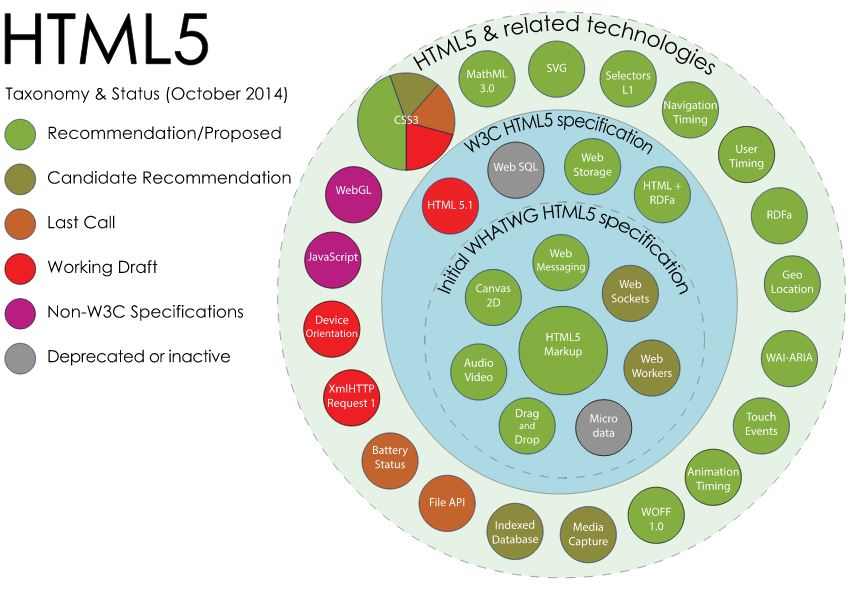
\includegraphics[width=0.7\linewidth]{obrazky/obrazokHTML}
\caption{HTML 5 API}
\label{fig:obrazokHTML}
\end{figure}
%http://html5.belisso.com/




%\ac*{W3C} značkový jazyk vždy bolo \acs{HTML}. 
%HTML bolo primárne navrhnuté ako jazyk, pre systematické opisovanie vedeckých dokumentov.  
%Hlavná oblasť
%TODO

%http://www.w3.org/TR/html5/  

%The World Wide Web's markup language has always been HTML. HTML was primarily designed as a language for semantically describing scientific documents, although its general design and adaptations over the years have enabled it to be used to describe a number of other types of documents.

%The main area that has not been adequately addressed by HTML is a vague subject referred to as Web Applications. This specification attempts to rectify this, while at the same time updating the HTML specifications to address issues raised in the past few years.

%1.2 Audience

%This section is non-normative.

%This specification is intended for authors of documents and scripts that use the features defined in this specification, implementors of tools that operate on pages that use the features defined in this specification, and individuals wishing to establish the correctness of documents or implementations with respect to the requirements of this specification.

%This document is probably not suited to readers who do not already have at least a passing familiarity with Web technologies, as in places it sacrifices clarity for precision, and brevity for completeness. More approachable tutorials and authoring guides can provide a gentler introduction to the topic.

%In particular, familiarity with the basics of DOM is necessary for a complete understanding of some of the more technical parts of this specification. An understanding of Web IDL, HTTP, XML, Unicode, character encodings, JavaScript, and CSS will also be helpful in places but is not essential.

%1.3 Scope
%
%This section is non-normative.

%This specification is limited to providing a semantic-level markup language and associated semantic-level scripting APIs for authoring accessible pages on the Web ranging from static documents to dynamic applications.

%The scope of this specification does not include providing mechanisms for media-specific customization of presentation (although default rendering rules for Web browsers are included at the end of this specification, and several mechanisms for hooking into CSS are provided as part of the language).

%The scope of this specification is not to describe an entire operating system. In particular, hardware configuration software, image manipulation tools, and applications that users would be expected to use with high-end workstations on a daily basis are out of scope. In terms of applications, this specification is targeted specifically at applications that would be expected to be used by users on an occasional basis, or regularly but from disparate locations, with low CPU requirements. Examples of such applications include online purchasing systems, searching systems, games (especially multiplayer online games), public telephone books or address books, communications software (e-mail clients, instant messaging clients, discussion software), document editing software, etc.

%1.4 History


%
%blal 3.2.5.1 The id attribute
%
%The id attribute specifies its element's unique identifier (ID). [DOM]
%
%The value must be unique amongst all the IDs in the element's home subtree and must contain at least one character. The value must not contain any space characters.





\section{Čo je SVG?}
\ac{SVG} je štandardný formát pre vektorovú grafiku. Vektorová grafika je definovaná cez body, priamky, mnohouholníky, elipsy, krivky, alebo iné geometrické tvary.  

\acs{SVG} je jazyk na opísanie dvojrozmernej grafiky v   \ac*{XML}. Vďaka tomu, umožňuje reprezentáciu grafických informácii v kompaktnom a prenositeľnom tvare.
%SVG patrí do rodiny špecifikácií HTML 5.

 SVG povoľuje tieto tri typy grafických objektov: vektorové grafické tvary, obrázky a text. 
Grafické objekty môžu byť zoskupené, štylizované, zmenené, a kombinované do predošlých vrstiev objektov. 

SVG obrázky môžu byť dynamické a interaktívne. \ac*{DOM} pre SVG, ktoré zahŕňa celé XML DOM, a povoľuje priamočiaro a efektívnu vektorovú grafickú animáciu cez príkazy. TODO

Prispôsobiteľnosť SVG umožňuje zmeniť veľkosť grafického komponentu bez straty kvality vzhľadu. Čo umožňuje zobraziť responzívne na viacerých možných zariadení. 
SVG sa bude zobrazovať rovnako na rôznych platformách. Je kompatibilná s štandardmi \acs{HTML}5, ktoré navrhla \ac*{W3C}. 

%http://www.w3.org/Graphics/SVG/About.html

%SVG is a language for describing two-dimensional graphics in XML. SVG allows for three types of graphic objects: vector graphic shapes (e.g., paths consisting of straight lines and curves), images and text. Graphical objects can be grouped, styled, transformed and composited into previously rendered objects. Text can be in any XML namespace suitable to the application, which enhances searchability and accessibility of the SVG graphics. The feature set includes nested transformations, clipping paths, alpha masks, filter effects, template objects and extensibility.

%SVG drawings can be dynamic and interactive. The Document Object Model (DOM) for SVG, which includes the full XML DOM, allows for straightforward and efficient vector graphics animation via scripting. A rich set of event handlers such as onmouseover and onclick can be assigned to any SVG graphical object. Because of its compatibility and leveraging of other Web standards, features like scripting can be done on SVG elements and other XML elements from different namespaces simultaneously within the same Web page.
 
 
 \subsection{Podpora v webovom prehliadači}
 Súčasné prehliadače plne podporujú SVG elementy.
 V tabuľke je TODO - PREROBIM TO ESTE DO TABULKY 
 \begin{figure}
\centering
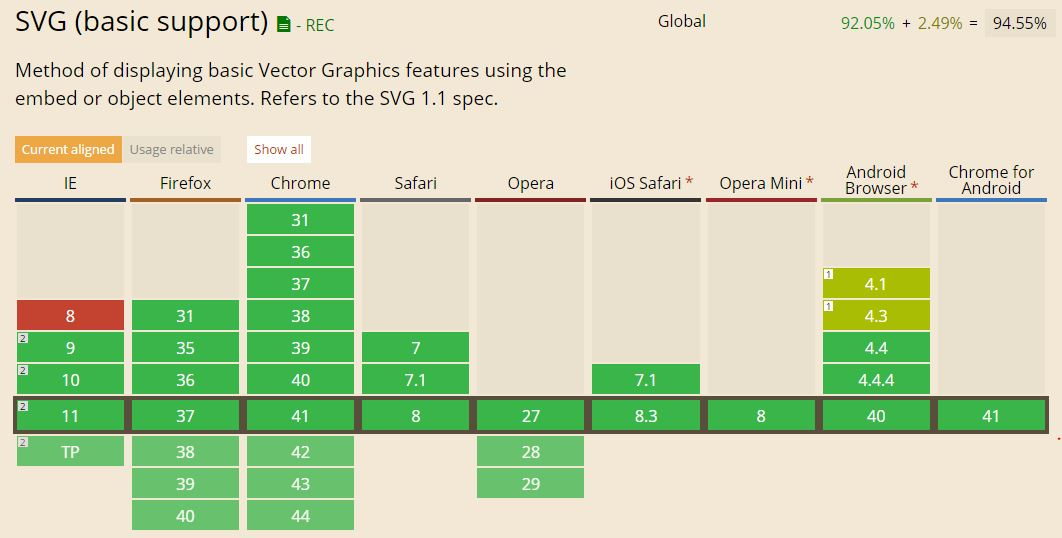
\includegraphics[width=0.7\linewidth]{obrazky/podpora}
\caption{podpora SVG vo webových prehliadačoch}
\label{fig:podpora}
\end{figure}

 
% http://caniuse.com/#feat=svg
 
 \subsection{Rozdiely medzi SVG a Canvas}
TODO \url{http://www.petrpexa.cz/diplomky/trantyr.pdf} strana 52


 SVG je jazyk na opisanie dvojrozmernej grafiky v XML. 
 Canvas kreslí dvojrozmernú grafiku za behu programu cez JavaScript.
 SVG je XML založený, čo znamená, že každý element je dostupný cez SVG DOM. Môžem k tomu priložiť JavaScript na ovládanie udalostí elementov. TODO . 
  %You can attach JavaScript event handlers for an element.
 V SVG je každý tvar zapamätaný ako objekt. Ak potrebujem zmeniť atribút SVG, tak prehliadač  automaticky prekreslí daný tvar.
 
 
 Canvas je prekresľovaný pixel za pixelom. Prehliadač na neho zabudne, ako náhle sa vykreslí. Keď chcem zmeniť jeho pozíciu, musím prekresliť úplne všetko. 
 
 
 %SVG is XML based, which means that every element is available within the SVG DOM. You can attach JavaScript event handlers for an element.
 %In SVG, each drawn shape is remembered as an object. If attributes of an SVG object are changed, the browser can automatically re-render the shape.
 %Canvas is rendered pixel by pixel. In canvas, once the graphic is drawn, it is forgotten by the browser. If its position should be changed, the entire scene needs to be redrawn, including any objects that might have been covered by the graphic.
 
 
 \subsection{Porovnanie Canvas a SVG}
 Tabuľka \ref{canvas:SVG} zobrazuje niekoľko dôležitých odlišností medzi Canvas a SVG. 
% The table below shows some important differences between Canvas and SVG:
 TODO DPI
 \begin{table}[h]
 \centering
 \begin{tabular}{|l|p{7.5cm} |}
 	\hline \textbf{Canvas} & \textbf{SVG} \\
 	 	\hline Závislé na rozlíšení a \acs{DPI} & Nezávislé na rozlíšení a DPI \\ 
 	\hline Nepodporuje dynamické zmeny & Podporuje dynamické zmeny \\ 
 	\hline Obmedzené možnosti na vykresľovanie  & Vhodné pre aplikácie s veľkými plochami na vykresľovanie \\ 
 	\hline & Väčší výpočtový výkon pri komplexnom obrázku \\ 
 	\hline Vhodné pre grafické-intenzívne hry & Nevhodné pre dynamické hry \\ 
 	\hline 
 \end{tabular} 

 \caption{Porovnanie Canvas a SVG}
 \label{canvas:SVG}
 
\end{table}
 
 
 \section{Základná syntax \acs*{SVG}}
TODO
V HTML5 sa môžu používať vložené SVG elementy priamo v na HTML stránke. 
%https://css-tricks.com/using-svg/

%TODO DOPLNIT POUTIZIIE TRI SPOSOBY \url{https://css-tricks.com/using-svg/}

SVG can be created 
-   inline: within the HTML document 
-   by embedding a stand alone .SVG file


Copy/paste SVG code within HTML code (inlining)
Using the HTML img tag
Using the HTML object tag
Using the HTML iframe tag
Using CSS (background images)
Including SVG within SVG using the image tag.


%citovane z knihy Sergey's HTML5 & CSS3 Quick Reference: HTML5, CSS3 and APIs (3rd Edition)
%preview je volne dostupny na nete / aspon tie kapitoly, ktore potrebujem


\begin{table}[h]
	\begin{center}
		\begin{tabular}{|l|l|}
			\hline \textbf{Technika} & \textbf{Popis} \\ 
			\hline $<$embed$>$ tag & Načíta vytvorený SVG súbor.  \\ 
			\hline $<$object$>$ tag & Nepovoľuje skriptovanie.  \\ 
			\hline $<$iframe$>$ tag & Zobrazí SVG v rámci  \\ 
			\hline Inline & Vytvorí Svg súbor \\ 
			\hline 
		\end{tabular} 
	\end{center}
	\caption{Spôsoby vytvorenia SVG v HTML dokumente}
	\label{vytvorenie:SVG}
\end{table}

Príklady načítania SVG v HTML dokumente.

$<$img$>$ tag 

\begin{lstlisting}
	Image:
	<img src="stanica2.svg" width = "50" height= "50" />
	
	Embed:
	<embed src="stanica2.svg" width = "50" height= "50" />
	
	Object:
	<object type="image/svg+xml" data="stanica2.svg"
	width="50" height="50"></object>
	
	Iframe:
	<iframe src="stanica2.svg" width = "50" height= "50"><</iframe>
	
\end{lstlisting}






\subsection{Príklad použitia SVG v HTML dokumentu s inline SVG }

HTML kód: 

\begin{lstlisting}
<!DOCTYPE html>
<html>
<head lang="sk">
<meta charset="UTF-8">
<title></title>
</head>
<body>

	<svg width="100" height="100">
		<circle cx="50" cy="50" r="40" stroke="black" stroke-width="2" fill="silver" />
	</svg>	
	
</body>
</html>

\end{lstlisting}




SVG obrázok začína s $<$svg$>$ elementom. Atribúty elementu $<$svg$>$ sú width a height. Definujú šírku a výšku SVG obrázka. Element $<$circle$>$ je použitý na nakreslenie kruhu. Atribúty cx, cy definujú x, y súradnice od centra kruhu. Ak je cx, cy vynechané, tak center kruhu je nastavený na $($0, 0$)$. Atribút r  definuje polomer kruhu. Atribúty stroke a stroke-width určujú to ako bude vyzerať obrys útvaru. Kruh má nastavený 2px čierny okraj. 
Atribút fill vyplní vnútro kruhu. V príklade je vyplnený sivou farbou. Tag, ktorý uzavrie SVG obrázok je $<$$/$svg$>$. Keďže SVG je validné XML, tak všetky elementy musia byť správne zatvorené. 
%zdroj www.w3schools.com/svg/svg_inhtml.asp


Vykreslí na HTML webovú stránku útvar, ktorý je na obrázku \ref{jednoduchyKruh}.

\begin{figure}[ht]
	\begin{center}
		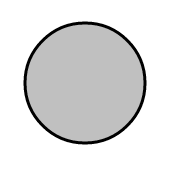
\includegraphics  {obrazky/jednoduchyKruh.png}
		\caption{Vykreslenie SVG na HTML stránke}
		\label{jednoduchyKruh}
	\end{center}
\end{figure}


\section{SVG útvary} 

\acs*{SVG} má preddefinované tieto tvary elementov:
\begin{itemize}
	\item Obdĺžník $<$rect$>$
	\item Kruh $<$circle$>$
	\item Elipsa $<$ellipse$>$
	\item Čiara $<$line$>$
	\item Polyline $<$polyline$>$
	\item Mnohouholník $<$polygon$>$
	\item Cesta $<$path$>$	
\end{itemize}

TODO ESTE NIECO PRIDAT

%\section{CSS vlastnosti - tuto kapitolu asi vyhodim}
%
%Podľa HTML5 štandardov dokáže CSS meniť vlastnosti SVG.
%
%%www.w3.org/tr/svg/styling.html
%%http://www.w3.org/TR/SVG/propidx.html http://www.w3.org/TR/SVG2/styling.html
%
%Vymenované vlastnosti, ktoré majú rovnaké \acs{CSS} 2.1 a \acs{SVG}. 
%
%Vlastnosti písma: 
%‘font’,
%‘font-family’,
%‘font-size’,
%‘font-size-adjust’,
%‘font-stretch’,
%‘font-style’,
%‘font-variant’,
%‘font-weight’.
%
%Vlastnosti textu: 
%‘direction’,
%‘letter-spacing’,
%‘text-decoration’,
%‘unicode-bidi’,
%‘word-spacing’.
%
%Ďalšie vlastností:
%‘clip’,
%‘color’ (‘fill’, ‘stroke’, ‘stop-color’, ‘flood-color’ a ‘lighting-color’), 
%‘cursor’,
%‘display’,
%‘overflow’,
%‘visibility’.
%
%Nasledujúce vlastností nie sú definované v CSS 2.1. 
%
%Clipping, Masking and Compositing properties:
%‘clip-path’, 
%‘clip-rule’,
%‘mask’, 
%‘opacity’.
%
%
%Filter Effects properties:
%‘enable-background’
%‘filter’
% ‘flood-color’
% ‘flood-opacity’
% ‘lighting-color’	
%
%
%Gradient properties: ‘stop-color’, 	‘stop-opacity’. 
%
%Interactivity properties:
%\begin{itemize}
%\item 	‘pointer-events’
%\end{itemize}
%Color and Painting properties:
%\begin{itemize}
%\item ‘color-interpolation’, ‘color-rendering’
%\item ‘fill’, ‘fill-opacity’, ‘fill-rule’
%\item ‘image-rendering’
%\item ‘marker’, ‘marker-end’, ‘marker-mid’,‘marker-start’
%\item ‘shape-rendering’
%\item ‘stroke’, ‘stroke-dasharray’, ‘stroke-dashoffset’, ‘stroke-linecap’, ‘stroke-linejoin’, ‘stroke-miterlimit’, ‘stroke-opacity’, ‘stroke-width’
%\item ‘text-rendering’	
%\end{itemize}
%
%Text properties:
%\begin{itemize}
%\item 	‘alignment-baseline’
%\item 	‘baseline-shift’
%\item 	‘dominant-baseline’
%\item 	‘glyph-orientation-horizontal’
%\item 	‘glyph-orientation-vertical’
%\item 	‘text-anchor’
%\item 	‘writing-mode’
%\end{itemize}
%
% 
%
%mozno tu este pridam nieco z prezentacii, ktore ma ucitel mikus
	%  
\chapter{Analýza požiadaviek}

\section{Nástroje na tvorbu grafických komponentov}

Našla som tieto \acs{WYSIWYG} editory, ktoré umožňujú tvorbu grafických komponentov: 

\begin{itemize}
\item Adobe Illustrator, 
\item CorelDraw, 
\item Inkscape,
\item Sketch, 
\item \url{http://www.drawsvg.org/} .
\end{itemize}

Nástroj, ktorý najviac vyhovuje mojim požiadavkam je Inkscape. 
Adobe Illustrator, CorelDraw, Sketch boli platené. 


%http://noeticforce.com/Javascript-libraries-for-svg-animation

\section{JavaScriptové knižnice pre grafické komponenty}
Na internete sa nachádzajú tieto OpenSource JavaScriptové knižnice na tvorbu grafických komponentov: 
\begin{itemize}
	\item \acs{D3}.js, 
	\item Raphael.js, 
	\item Snap.svg.js,  
	\item Svg.js. 
\end{itemize}



Popis jednotlivých JavaScriptových knižníc.

%\section{JavaScript knižnice SVG}


%http://christopheviau.com/d3_tutorial/d3_inkscape/
\subsection{D3.js}
D3  - \textbf{D}ata \textbf{D}riven \textbf{D}ocument -  dostupné na: \url{http://d3js.org/}.

D3.js je JavaScriptová knižnica určená na manipuláciu dokumentov vychádzajúcich z dátach. Pomocou \acs{HTML}, \acs{SVG} a \acs{CSS} umožňuje TODO vdýchnuť život dátam. 
Je veľmi vhodná na vytváranie interaktívnych SVG grafov s hladkými prechodmi a interakciami. 

%D3.js is a JavaScript library for manipulating documents based on data. D3 helps you bring data to life using \acs{HTML}, \acs{SVG} and \acs{CSS}. D3’s emphasis on web standards gives you the full capabilities of modern browsers without tying yourself to a proprietary framework, combining powerful visualization components and a data-driven approach to DOM manipulation. 

%D3 allows you to bind arbitrary data to a ac*\{DOM}, and then apply data-driven transformations to the document. For example, you can use D3 to generate an HTML table from an array of numbers. Or, use the same data to create an interactive SVG bar chart with smooth transitions and interaction.

D3 rieši efektívnu manipuláciu dokumentov zakladajúcich si na dátach. Využíva webové štandardy ako \acs{HTML}, \acs{SVG} a \acs{CSS}3. 

%D3 is not a monolithic framework that seeks to provide every conceivable feature. Instead, D3 solves the crux of the problem: efficient manipulation of documents based on data. This avoids proprietary representation and affords extraordinary flexibility, exposing the full capabilities of web standards such as CSS3, HTML5 and SVG. With minimal overhead, D3 is extremely fast, supporting large datasets and dynamic behaviors for interaction and animation. D3’s functional style allows code reuse through a diverse collection of components and plugins. 

\subsection{Raphaël.js}
Raphael.js je dostupné na: \url{http://raphaeljs.com/}.
%mohla by som spomenut kto ju vytvoril

Raphaël je malá JavaScriptová knižnica, ktorá umožnuje jednoducho pracovať s vektorovou grafikou na webe. Umožňuje pomocou jednoduchých príkazov vytvárať špecifické grafy, obrázky. 

%Raphaël is a small JavaScript library that should simplify your work with vector graphics on the web. If you want to create your own specific chart or image crop and rotate widget, for example, you can achieve it simply and easily with this library.
Raphaël využíva \acs{SVG} \acs{W3C} odporúčania a \acs{VML} na tvorbu grafických komponentov. Z toho vyplýva, to že každý grafický objekt, ktorý vytvorím je zároveň aj DOM objekt. To umožnuje cez JavaScriptové pridávať manipuláciu udalostí, alebo upravovať ich neskôr.
Momentálne podporuje Firefox 3.0+, Safari 3.0+, Chrome 5.0+, Opera 9.5+ and Internet Explorer 6.0+.
Autor knižnice je Dmitry Baranovskiy. 


%Raphaël  uses the SVG W3C Recommendation and VML as a base for creating graphics. This means every graphical object you create is also a DOM object, so you can attach JavaScript event handlers or modify them later. Raphaël’s goal is to provide an adapter that will make drawing vector art compatible cross-browser and easy.

%Raphaël currently supports Firefox 3.0+, Safari 3.0+, Chrome 5.0+, Opera 9.5+ and Internet Explorer 6.0+. 


\subsection{Snap.svg.js}

Snap.svg.js \url{http://snapsvg.io/}

Je JavaScriptová knižnica na prácu s SVG. Poskytuje pre webových developerov \acs{API}, ktorá umožňuje animáciu a manipulovanie s buď existujúcim SVG, alebo vygenerovaným s Snapom. 

Snap bol napísaný rovnakým autorom ako Raphael.  Bola navrhnutá špeciálne pre moderné prehliadače (IE9 a vyššie, Safari, Chrome, Firefox, and Opera). Z toho vyplýva, že umožňuje podporu maskovania, strihania, vzorov, plných gradientov, skupín... 

%Snap.svg is a brand new JavaScript library for working with SVG. Snap provides web developers with a clean, streamlined, intuitive, and powerful API for animating and manipulating both existing SVG content, and SVG content generated with Snap.

%Currently, the most popular library for working with SVG is Raphaël. One of the primary reasons Raphaël became the de facto standard is that it supports browsers all the way back to IE 6. However, supporting so many browsers means only being able to implement a common subset of SVG features. Snap was written entirely from scratch by the author of Raphaël (Dmitry Baranovskiy), and is designed specifically for modern browsers (IE9 and up, Safari, Chrome, Firefox, and Opera). Targeting more modern browsers means that Snap can support features like masking, clipping, patterns, full gradients, groups, and more.

Medzi hlavnú výhodu považujem schopnosť pracovať s existujúcim SVG súborom. To znamená, že nemusím SVG obsah generovať cez Snap, aby som ho mohla používať. Z toho vyplýva, že môžem vytvoriť SVG obsah v nástroji ako Illustrator, Inkscape, alebo Sketch a potom animovať, alebo inak manipulovať cez Snap. Môžem pracovať aj s reťazcom SVG.

%Another unique feature of Snap is its ability to work with existing SVG. That means your SVG content does not have to be generated with Snap for you to be able to use Snap to work with it (think “jQuery or Zepto for SVG”). That means you create SVG content in tools like Illustrator, Inkscape, or Sketch then animate or otherwise manipulate it using Snap. You can even work with strings of SVG (for example, SVG files loaded via Ajax) without having to actually render it first which means you can do things like query specific shapes out of an SVG file, essentially turning it into a resource container or sprite sheet.

Snap podporuje animácie. Poskytuje jednoduché a intuitívne JavaScript API pre animáciu. Snap umožňuje urobiť SVG obsah viac interaktívnejší a záživnejší. 
%Snap je zadarmo a open-source. 

%Finally, Snap supports animation. By providing a simple and intuitive JavaScript API for animation, Snap can help make your SVG content more interactive and engaging.

%Snap is    free and   open-source (released under an Apache 2 license).

\subsection{SVG.JS}
\url{http://www.svgjs.com/}
Ďalšia knižnica umožňujúca manipulovať a animovať SVG.

Medzi hlavné výhody knižnice patrí to, že je má ľahko čitateľnú syntax. Umožňuje animovanie veľkosti, pozície, transformácie, farby. Má modulárnu štruktúru, čo umožnuje používanie rôznych rozšírení. Existuje množstvo užitočných pluginou dostupných na internete. 

%A lightweight library for manipulating and animating SVG. 
%
%\begin{itemize}
%	\item easy readable uncluttered syntax
%	\item    animations on size, position, transformations, color, ...
%	\item   painless extension thanks to the modular structure
%	\item various useful plugins available
%	\item unified api between shape types with move, size, center, ...
%	\item binding events to elements
%	\item full support for opacity masks and clipping paths
%	\item text paths, even animated
%	\item   element groups and sets
%	\item   dynamic gradients
%\end{itemize}

\section{Zhodnotenie požiadaviek}
Grafické komponenty budem vytvárať v programe Inkscape. Ovládanie a animovanie prostredníctvom knižnice Snap.svg.js. Hlavný dôvod, prečo som sa rozhodla pre túto knižnicu bol, že dokáže načítavať SVG súbor a potom s ním manipulovať.
Spĺňa požiadavku kompatibility pre moderné webové prehliadače. Je to open-source knižnica a má licenciu Apache 2.  	%  
\chapter{Popis vytvorenia SVG v Inkscape}

Vytvorenie SVG v programe Inkscape .


\begin{figure}[ht]
	\begin{center}
		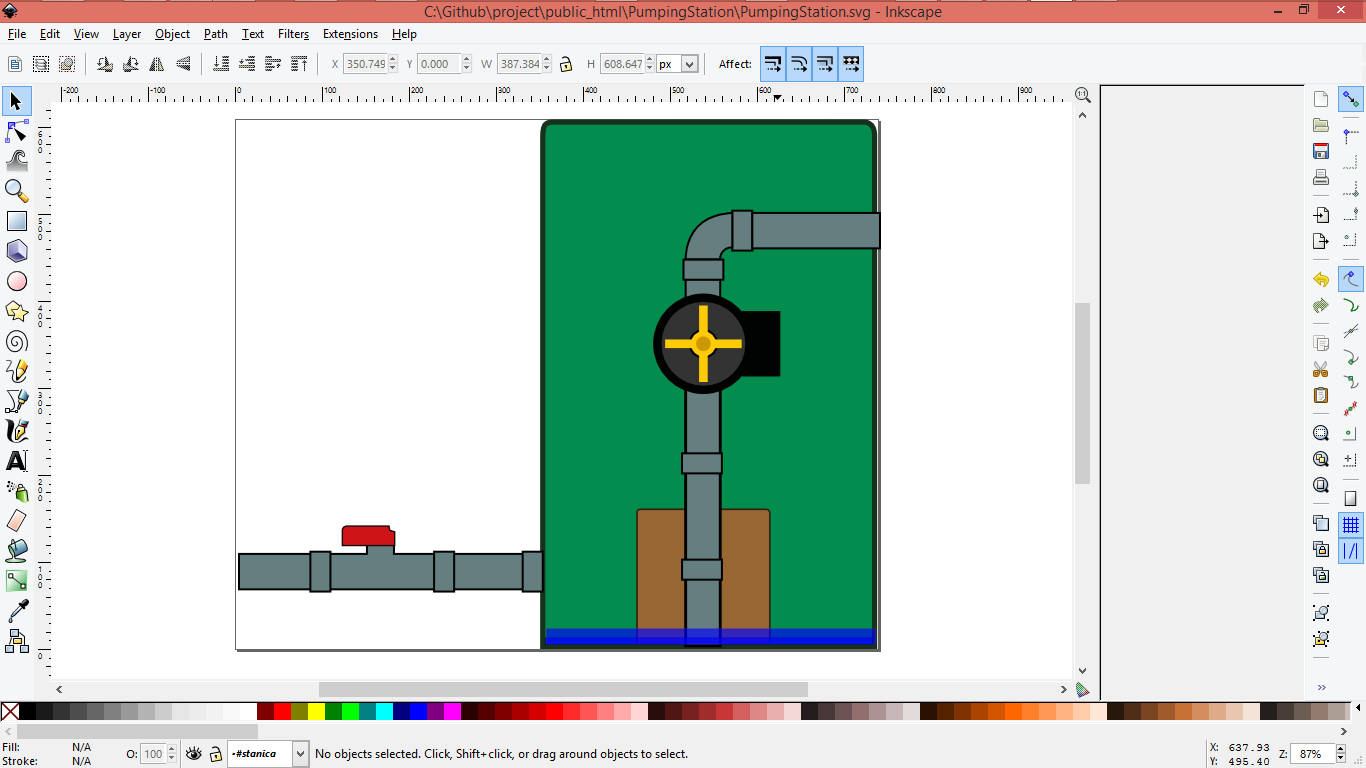
\includegraphics [width=12.5cm] {obrazky/obr1.png}
		\caption{obrázok 1}
		\label{picture1}
	\end{center}
\end{figure}

Nakreslenie jednotlivých častí komponentov pomocou bočného panela. 

Pre ovládanie JavaScriptom je nutné si pozrieť jednotlivé ID SVG Klikneme pravým tlačidlom na daný komponent, časť, a potom na Objekt Properties.

\begin{figure}[ht]
	\begin{center}
		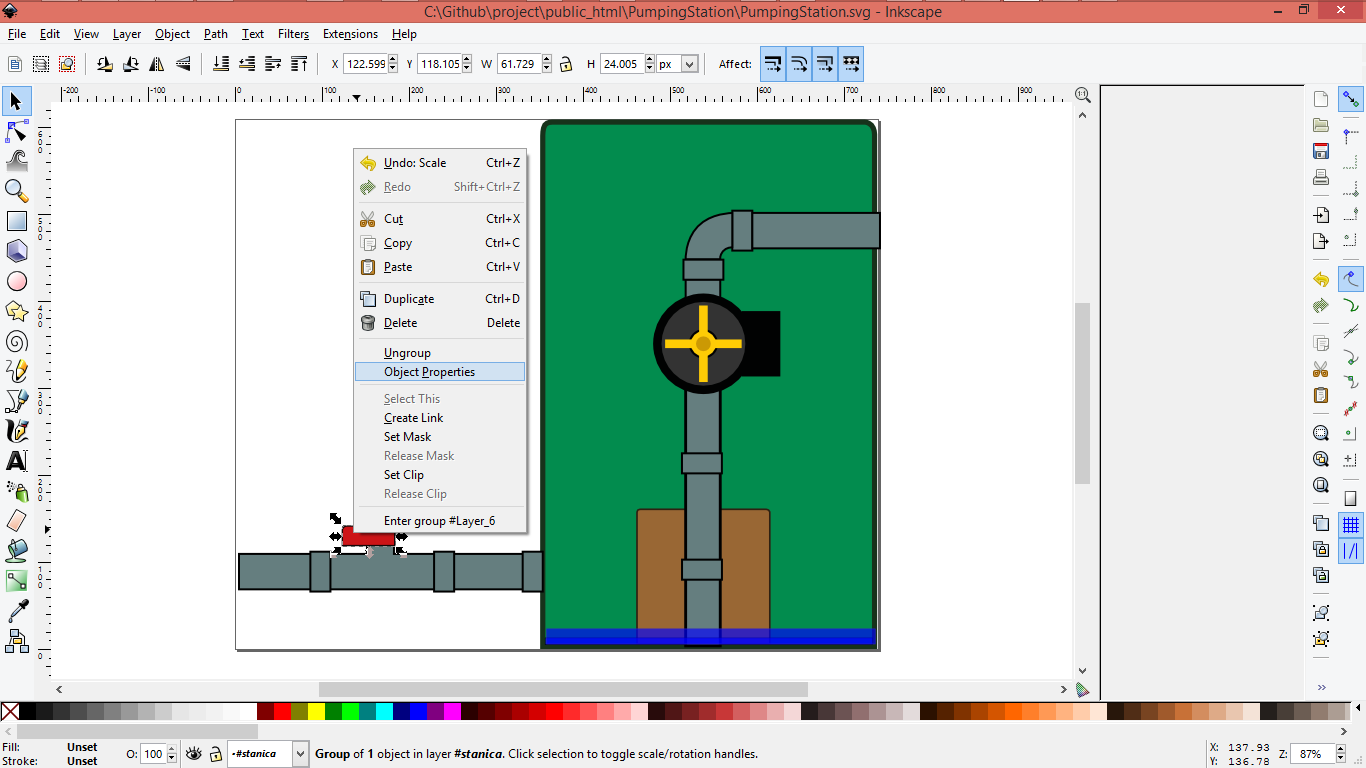
\includegraphics [width=12.5cm] {obrazky/obr2.png}
		\caption{obrázok 2}
		\label{picture2}
	\end{center}
\end{figure}

Zobrazí sa nám nasledovné okno obrázok č.x. 

\begin{figure}[ht]
	\begin{center}
		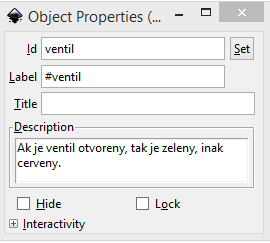
\includegraphics  {obrazky/obr3.png}
		\caption{obrázok 3}
		\label{picture3}
	\end{center}
\end{figure}


Z obrázka možno vyčítať aké je ID, predvolené sú tam napr. desc3072. Hodnoty je možné zmeniť tlačidlom Set. Pre nás je dôležitá hodnota v kolónke Label - \#ventil. Toto nám umožni potom neskôr ako CSS selektor, cez ktorý budeme môcť ovládať danú časť. Spravidla hodnoty ID a Label sú rovnaké, a líšia sa iba v \#. ID je unikátny názov pre danú vetvu SVG 

Alebo ďalší spôsob zistenia ID SVG je priamo nájsť tú hodnotu v nazovSuboru.SVG Je to označené ako ID="ventil" .

\begin{figure}[ht]
	\begin{center}
		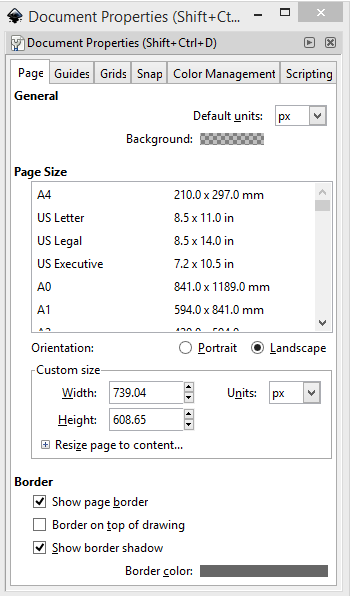
\includegraphics  {obrazky/obr4.png}
		\caption{obrázok 4}
		\label{picture4}
	\end{center}
\end{figure}

Plná nádrž ma nasledovne parametre:

\begin{figure}[ht]
	\begin{center}
		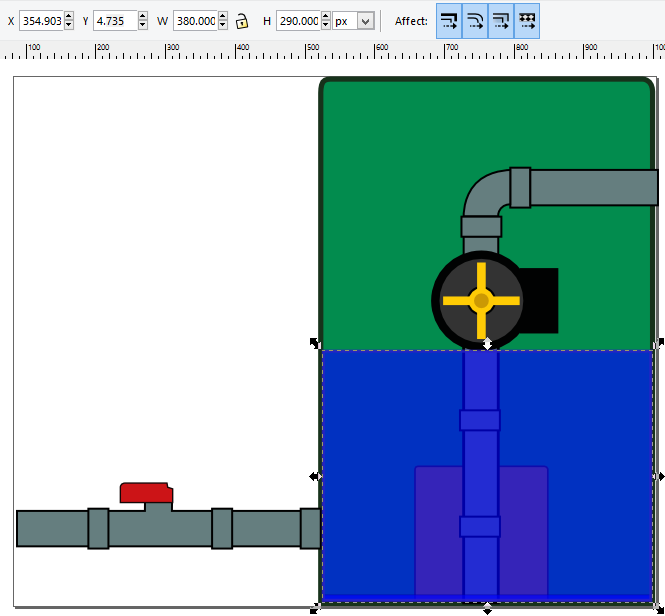
\includegraphics [width=10cm]  {obrazky/obr5.png}
		\caption{obrázok 5}
		\label{picture5}
	\end{center}
\end{figure}

V SVG súbore je to 
\begin{verbatim}

Inkscape:label="\#hladina"
y="1320.1689"
x="2507.8459"
height="605.83868"
width="797.04492"
id="hladina"
\end{verbatim}


Prázdna nádrž
\begin{figure}[ht]
	\begin{center}
		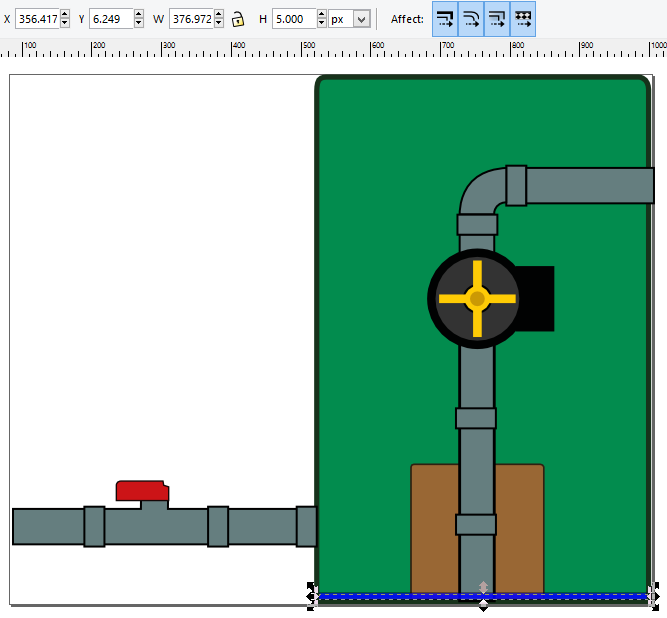
\includegraphics [width=10cm]  {obrazky/obr6.png}
		\caption{obrázok 6}
		\label{picture6}
	\end{center}
\end{figure}

v SVG to je nasledovne 
\begin{lstlisting}[language=html]
<rect
inkscape:label="\#hladina"
y="1916.3605"
x="2507.8459"
height="9.6471272"
width="797.04492"
id="hladina"
...
\end{lstlisting}



Hladina nádrže:
vykreslená ako obdĺžnik
\begin{lstlisting} [language=html]
<rect
	inkscape:label="#hladina"
	y="1320.1689"
	x="2507.8459"
	height="605.83868"
	width="797.04492"
	id="hladina"
	style=
		"fill:#0000ff;
		fill-opacity:0.65098039;
		fill-rule:evenodd;
		stroke:#2c20c8;
		stroke-width:7.42523718px;
		stroke-linecap:butt;
		stroke-linejoin:miter;
		stroke-opacity:0.80952382">
<desc id="desc3119-4">hladina</desc>
<title id="title3117-0">hladina</title>
</rect>
\end{lstlisting}


Parametre ako stroke, fill, a iné sa dajú meniť prostredníctvom attr v Snap. … TODO

	%  
\chapter{Implementácia komponentov}

Keď už máme nakreslený komponent pomocou Inkscape, tak postupujem dalej. TODO

Pridáme do HTML  
\begin{lstlisting}
<svg  
	id="svgStanica"  
	viewBox="0 0 750 600" 
	width="40%" 
	height="40%" 
	>
</svg>
\end{lstlisting}


id / toto pouzijeme pri vykresleni 
viewBox - je atribút, ktorý povoľuje špecifikovať danú množinu grafick.. aby to fit a vošlo do kontajnera elementu. Hodnoty atribútov v viewBox sú štyri čísla - min-x, min-y, width a height. 
Width a height je šírka a výška - a je možné ich uviesť aj relatívne v percentách, alebo absolútne v pixeloch. 

\begin{lstlisting}


<body onload="onPageLoad();">

function onPageLoad() {
	PumpingStation("PumpingStation.svg", "#svgStanica" );
}
\end{lstlisting}
Parametre pre PumpingStation je nazov svg suboru, a tag v html.
\begin{lstlisting}
var PumpingStation = function(nazovFileSVG, nameHTMLidSVG) \{
	paper = Snap(nameHTMLidSVG);
	Snap.load(nazovFileSVG, function (f) \{
		paper.append(f);
\});
\};
\end{lstlisting}
paper - bude globalna premenna. Vytvorí plochu na  kreslenie, alebo  wraps existujúci SVG element. Ako parametre môžu byť buď šírka, výška, alebo DOM element. 

Pomocou load nacitam svg subor, ktory som vytvorila a pomocou append ho zobrazim na danu plochu. 

\subsection{Tank}
Zanimovanie stupania a klesania hladiny nadrze. 
\begin{lstlisting}
var Tank = {
	idTank: "#hladina",
	tank: function(){
		return  paper.select(this.idTank);},
	animateComponentTank: function(fillPerc) {
		if (fillPerc === undefined || fillPerc < 0) {
			fillPerc = 0;
		}
		var perHeight = 600 * (fillPerc / 100);
		var perY = 1912 - perHeight;
		this.tank().animate  (	{
			height: perHeight,
			y: perY
		}, 800);
		return console.log("animacia tanku " + fillPerc);
	}
};
\end{lstlisting}
Vytvorila som objekt Tank medzi jeho atributy patria: idTank, funkcia tank, a animateComponentTank. IdTank - je stringové - je to id, ktoré som získala zo svg súboru, alebo cez Inkscape ako Label. Funkcia tank - vyberie dany objekt, ktory chcem ovladat. Pomocou Tank.tank() mozem volat funkcie z Snap kniznice. n 

Zanimovanie tanku je realizovane v funkcii animateComponentTank - kde parametrom je v percentách udane o koľko sa ma zdvihnut hladina nadrze. 
Využívam funkciu animate. Kde v prvom parametri - mením výšku a os y. Hodnotu perHeight je výška 600, ktoru vynásobím percentom o ktore sa ma posunut. PerY je hodnota, o ktoru sa posunei po y-osi. Je vypocitana ako 1912 co je y prázdnej nádrže a je od nej odpocitana hodnota vysky. 
Dalsi parameter pri funkcii animate() je rýchlosť animácie vyjadrená v milisekundach. 

\subsection{Ventil}

\begin{lstlisting}
var Valve = {
	idValve: "#ventil",
	valve: function (){ return paper.select(this.idValve);},
	colorValve: "red",
	changeIsOpen: function (isOpened) {
		isOpened = (isOpened) ? 0 : 1;
		this.colorValve = (isOpened) ?   "red" : "green";
		this.valve().attr({fill: this.colorValve});
		return;);
	}
}
\end{lstlisting}

Farba sa dá zmeniť aj príkazom 

\begin{verbatim}
Valve.valve().attr({fill: “green”});.
\end{verbatim}

Názov farby môže byť uvedený slovne, alebo ako RGB. 

Zmena farby Valve - \begin{verbatim} this.valve().attr  ({fill: this.colorValve}); \end{verbatim}

	%  
\chapter{Návrh \acs{REST} \acs{API}}

%JSON

%23 strana knihy restful web apis

\section{\acs{JSON}}


%%
%\ac{JSON} predstavuje spôsob, ako poskytovať objekty JavaScriptom ako dáta namiesto kódovania týchto dát do dokumentu XML. ....TODO

TODO PREROBIT CELE - TODO - 
%Formát \ac{JSON} je založený na rovnakom princípe ako sa tvoria objekty v JavaScripte. Dátový formát je schopný reprezentovať rovnaké typy dát ako jazyk \acs{XML}. \cite[p.~622-4]{Zakas}

%JSON je efektívnejší spôsob ako posielať dáta od serveru klientovi, pretože nie je potrebné spracovať odpoveď pomocou \acs{DOM} a dáta je možné použiť ihneď, bez nutnosti explicitnej konverzie na objekty JavaScriptu. \cite[p.~280]{Suehring}







%\subsection{JSON Syntax}




%Napríklad ko  
%
%Pravidlá pre tvorbu JSON:
%
%\begin{itemize}
%	\item Dáta sú pároch - meno/hodnota 
%	\item Dáta musia byť v úvodzovkách, napríklad "fillPerc":"50"
%	\item Dáta sú oddelené čiarkou
%	\item Kučeravé zátvorky uchovávajú objekty
%	\item Hranaté zátvorky ukladajú pole
%	\item Nemôže obsahovať komentáre
%	\item 
%\end{itemize}

%štandard - pre JSON
%http://www.ecma-international.org/publications/files/ECMA-ST/Ecma-262.pdf


API k Pumping station schéme. 

\begin{lstlisting}
var updateData = {
	"valve": "true",
	"tank": "20",
	"engine": "20"
};
\end{lstlisting}

Tento kód definuje objekt s názvom updateData, ktorá má tri vlastnosti. 




 Interface funkcia k REST API. 
 
 \begin{lstlisting}
 function updateSchema(updateData){
	 updateSchema01(updateData.valve, updateData.tank, updateData.engine);
 }
 \end{lstlisting}
	%  Zaver



%%%%%%%%%%%%%%%%%% literatura


%%%%%%%%%%%%%%%%%%%%%%%%%%%%%%%%%%%%%%%%%%%%%%%%%%%%%%%%%%%%%%%%%%%%%%%%%%%%%
\begin{thebibliography}{99}                               
	 \label{literatura}
%\addcontentsline{toc}{section}{Literatúra}
%\addcontentsline{toc}{chapter}{Zoznam použitej literatúry}




\bibitem{Dawber}
Dawber D.,
{\it Learning Raphael JS Vector Graphics }, 
 Packt Publishing, 2013, ISBN 978-1-78216-916-1
         
 
 
\bibitem{Wilson} Wilson CH., {\it RaphaelJs Graphic and visualization on the web} , 
O'Reilly Media, 2013, ISBN 978-1-449-36536-3
         

\bibitem{Haverbeke}
Haverbeke M., 
{\it Eloquent Javascript} 2. vyd. No Starch Press, 2014, ISBN 978-1-59327-584-6


\bibitem{Zakas}
Zakas N. Z., 
{\it JavaScript pro webové vývojáře Programujeme profesionálně},
 v1. vyd. Brno:Computer Press, a.s., 2009,  ISBN 978-80-251-2509-0

\bibitem{Suehring}
Suehring S., 
{\it JavaScript krok za krokem},
1. vyd. Brno:Computer Press, 2008, ISBN 978-80-251-2241-9

\bibitem{ZakasA}
Zakas N. C., McPeak J., Fawcett J.,
{\it Profesionálně Ajax},
Zoner Press, 2007,  ISBN 978-80-86815-77-0

\bibitem{Eisenberg}
Eisenberg D. J., {\it SVG Essentials}, 
O'Reilly Media 2002, ISBN  978-0-596-00223-7,  dostupné na \url{http://commons.oreilly.com/wiki/index.php/SVG_Essentials}

\bibitem{Richardson}
Richardson L., Amundsen M., {\it RESTful Web APIs} 
1. vyd. O'Reilly Media, 2013, 
ISBN 978-1-449-35806-8

\bibitem{Allamaraju}
Allamaraju S., {\it RESTful Web Services Cookbook} 
1. vyd. O'Reilly Media, 2010, 
ISBN 978-0-596-80168-7

\bibitem{snapsvg}
The JavaScript SVG library for the modern web,
\url{http://snapsvg.io/}.


\bibitem{Raphael}
\url{ http://raphaeljs.com/}

\bibitem {d3js}
\url {http://d3js.org/}

%\bibitem{snapsvg}
% \url{http://snapsvg.io/}
 
 \bibitem{svgjs}
 \url{http://www.svgjs.com/}


\bibitem {Inkscape}
Inkscape is a professional vector graphics editor for Windows, Mac OS X and Linux. It's free and open source.
\url {http://www.inkscape.org/en/about/features/}

\end{thebibliography}	%  Literatura


\end{document}


